\section{Computing Clearance Value Annotations}
\label{aha:planningwithannotations}
On a grid map, a clearance value is perhaps best explained as representing the length or width of a square that begins at some octile being evaluated and is expanded symmetrically to the right and down until it intersects an obstacle.     
To make our ideas more concrete we will use as a running example a simple environment featuring two terrain types: Ground (represented as white tiles) and Trees (represented as grey tiles). To distinguish traversable tiles from non-traversable tiles we will colour hard obstacles black. 
The set of capabilities, $C$, required to traverse such a map is thus defined as $C = {{Ground}, {Trees}, {Ground \wedge Trees}}$.
\par \indent
Figure \ref{aha-fig:annotations} (a) to (e) illustrates how clearance can be computed with an iterative procedure in an environment as described above.
In fig. \ref{aha-fig:annotations}(a) the clearance square for the highlighted traversable target tile is initialised to 1. 
Subsequent iterations (fig \ref{aha-fig:annotations}(b)-(c)) extend the square and increment the clearance. 
The process continues until the square contains an obstacle (fig. \ref{aha-fig:annotations}(d)) or extends beyond a map boundary at which point we terminate and do not increment clearance any further.
\par \indent
In fig. 1(e) we show the resultant clearance values for the single-terrain ${Ground}$ capability on a toy map example (note that we omit zero-value clearances).
Similarly, figures 1(f) and (g) show the clearance values associated with the ${Trees}$ and ${Ground \wedge Trees}$ capabilities respectively.  

\begin{figure}[htbp]
       \caption{\emph{(a)-(d) The annotation process. (e)-(g) Clearance values for different capabilities.}}
       \begin{center}
                       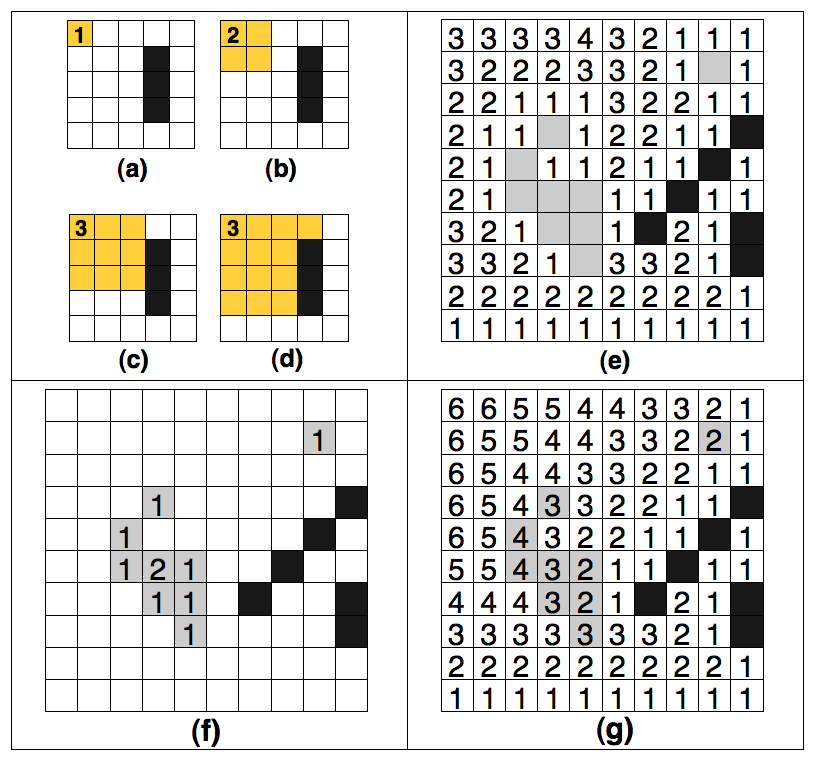
\includegraphics[scale=0.25]{diagrams/annotations.png}
       \end{center}
       \label{aha-fig:annotations}
\end{figure}

Once a clearance value is derived we store it in memory and repeat the entire procedure for each $c \in C$. The algorithm terminates when all octiles $t \in gridmap$ have been considered. 
We omit precise implementation details of where to store clearances as these considerations will vary depending on the specific application and available resources. We opted to add attributes to our node data structures for simplicity; a better method would be to use compact tables.
\par \indent
We can characterise the space complexity associated with computing clearance values in this fashion as so:
\begin{lemma}
\label{aha-lemma:numannotations}
Let $r$ be the number of all terrain types in an environment, $V$ the set of all graph vertices and $V_{HO} \in V$ the set of hard obstacles. Then, the number of clearance values required for a non-abstract graph is $|V|*2^r/2 - |V_{HO}|$
\end{lemma}

\begin{proof}
For a node to be traversable for some capability, the capability must include the node's terrain type (by definition). 
There are $2^r$ capabilities (by induction) but the maximum number of capabilities that include a node's terrain type is $2^r/2$ (by induction). 
There are $|V|$ nodes in total to represent the envrionment, and we avoid storing any clearance values for all nodes in $V_{HO}$. 
\qed
\end{proof}

The result from lemma \ref{aha-lemma:numannotations} suggests that it is impractical to store every clearance value; there are $\Theta(2^r)$ per node.
Luckily, clearance values can be computed on-demand with little effort. 
We present such an approach in algorithm \ref{aha-alg:calculateclearance}. 
It is worth noting that the amount of time required to determine clearance for an octile can be further reduced if the size of the agent is known beforehand; in such cases, we need only consider the tiles inside a clearance square of maximum area $s^2$ octiles.
\input algorithms/alg1_calculateclearance
\par \indent
The key advantage of annotating a map in this fashion is that we are able to plan for both large and small agents using a fixed size grid. We present the following theorem and proof by construction to demonstrate the validity of this claim:
\begin{theorem}
\label{aha-theorem:reducibility}
Given an annotated grid map, any instance of a large-agent search problem can be reduced into a small-agent search problem, where the size of the agent is one tile.
\end{theorem}

\begin{proof}
A clearance value for some tile $t \in gridmap$ is given by $t(c_{t}) = cv$ and measures the distance to the nearest obstacle for some capability $c_{t} \in C$ by taking the height or width of a maximal-size clearance square (by definition). 
If $cv > 0$ it must be the case that the terrain type of every tile in the clearance square is included in $c_{t}$ (by definition). 
\par \indent
For an agent to traverse a tile it must have a size $s$ and capability $c_{a} \in C$ such that $t(c_{a}) \geq s$ (intuitively).
If this condition holds, it must be the case that every tile in the area that will be occupied by the agent is traversable for that agent (by induction). 
Thus, a large agent is able to navigate across a map by only considering the traversal requirements of the top-left node it will occupy. \qed
\end{proof}
This is a highly useful result because it indicates that we can apply abstraction techniques from classical path planning to answer much more complex queries involving a wide range of terrain type and agent-size variables.
